%        File: wm_2013_nuc.tex
%     Created: Mon Aug 13 10:00 AM 2012 C
%
\documentclass[letterpaper, 11pt]{article}
\usepackage[top=1.0in,bottom=1.0in,left=1.0in,right=1.0in]{geometry}
\usepackage{amssymb}
\usepackage{graphicx}
%\usepackage{amsfonts}
\usepackage{amsmath}
\usepackage[usenames]{color}
\usepackage[
naturalnames = true, 
colorlinks = true, 
linkcolor = Black,
anchorcolor = Black,
citecolor = Black,
menucolor = Black,
urlcolor = Blue
]{hyperref}
\def\thesection       {\arabic{section}}
\def\thesubsection     {\thesection.\alph{subsection}}
\newcommand{\Cyclus}{\textsc{Cyclus}}
% For WMSym (Eqn. #) requirement :
\renewcommand{\theequation}{Eqn. \arabic{equation}}
% For the header to say all the stuff WMSym  needs :
\usepackage{fancyhdr}
\setlength{\headheight}{15.2pt}
\pagestyle{fancy}
\lhead{WM2013 Conference, February 24-28, 2013, Phoenix, Arizona, USA}
\rhead{}
\renewcommand{\headrulewidth}{0pt}
% So that the title is closer to the header : 
\usepackage{titling}
\setlength{\droptitle}{-0.75in}
% So that the title font is not bigger than 12pt
\newcommand*{\TitleFont}{%
      \fontsize{11}{13}%
      \selectfont}
% So that the section font is not bigger than 12pt
\usepackage{titlesec}
\titleformat{\section}{\fontsize{11}{13}\bfseries}{\thesection}{1em}{}

% No paragraph indentation
\setlength{\parindent}{0pt}

\author{\TitleFont Kathryn D. Huff
\\\TitleFont Argonne National Laboratory, 9700 S. Cass Ave, Argonne, IL. khuff@anl.gov
}

\date{}

% concise yet adequately descriptive title
\title{\TitleFont Hydrologic Nuclide Transport Models in Cyder, A Geologic Disposal Software Library - 13328}
\begin{document}
\maketitle
% So that the header shows up on the first page too.
\thispagestyle{fancy}


% 1) a descriptive title that will reflect the paper 
%    and presentation content (define all acronyms); 
% 2) a summary of the work conducted, 
%    problem history and your results; 
% 3) all authors contact information including mailing address, email addresses and phone 
%    numbers; and 
% 4) a brief description of the importance of the work 
%    (what problem it addresises/solves) and its application/benefit to others.  


% Abstracts should be between 400 - 800 words and comply with the 
% criteria stated below. Results have shown that brief abstracts that fully and 
% effectively convey the substance and their importance have the highest 
% ranking. Background information irrelevant to an abstract’s merits may 
% dilute the substance and lower the ranking. The evaluation criteria on the 
% “Abstract Rating Form” is posted on the WM website www.wmsym.org
% under the Presenters tab as a guide for authors. Insufficient information 
% for the reviewers may result in session misplacement, lower ranking or 
% abstract rejection.

% Some analytical models have been created for cyder, many levels of detail 
% % Degradation Rate
% % Mixed Cell 
% % Lumped Param
% % OneDimPPM
% Some sensitivity analyses have been conducted to improve the speed 
% % gdsm
% % what params
% %  
% % 
% They've been implemented in a flexible, modular way. 


% 2. How is the technical problem, issue or program and its importance clearly described?                    
% 3. How are the results or likely results of the investigation/solutions(s) to the problem or 
%    issue described?
%    5 - Very clearly described and supported
%    4 - Above-average
%    3 - Average and somewhat unfocused in specific details
%    2 - Below-average
%    1 - Abstract lacks a clear issue, focus and/or results
% 4. What is the significance of the work/results described?               
%    4 - Significant and widely applicable
%    3 - Applicable to a previously difficult or specific problem or issue resolution
%    2 - Incremental improvement to/status update of an already solved problem      
%    1 –Addresses an already resolved problem     
%    0 - Addresses no known or significant problem or issue by the reviewer
%5. Is the work original and new or an expansion of prior work?             
%    2 – Presents new work/results or new insight
%    1 - Effectively builds on previous work/results
%    0 - Nothing significantly new in work, program, issue resolution or results
%6. How is the information discussed likely to be of interest to attendees? 
%    4 - Will provide an excellent presentation and be a benefit to attendees
%    3 - Will provide an above-average presentation
%    2 - Will result in an average presentation
%    1 - Will be a below-average presentation
%7. Total of the Individual Reviewer’s Scores
\vspace{-0.5in}
\section*{ABSTRACT}

Component level and system level abstraction of detailed computational geologic 
repository models have resulted in four rapid computational models of hydrologic 
radionuclide transport at varying levels of detail. Those models are described, 
as is their implementation in Cyder, a software library of 
interchangeable radionuclide transport models appropriate for representing 
natural and engineered barrier components of generic geology repository 
concepts. A proof of principle demonstration was also conducted in which these models 
were used to represent the natural and engineered barrier components of a 
repository concept in a reducing, homogenous, generic geology. 
This base case demonstrates integration of the Cyder open source library with the Cyclus 
computational fuel cycle systems analysis platform to facilitate calculation of
repository performance metrics with respect to fuel cycle choices.

\section*{INTRODUCTION}
% Provide a summary of the work conducted:
%      Describe the technical problem clearly
%      support it with a method
% SubSection: Motivation
% Provide a brief description of the importance of the work (what problem it 
%   addresses/solves):
Radionuclide containment behavior of a geologic repository is a strong function 
of spent fuel composition, which varies among alternative fuel cycles. For this 
reason, a generic disposal model capable of integration with a systems analysis 
framework is necessary to illuminate performance distinctions of candidate 
repository geologies, designs, and engineering components in the context of fuel 
cycle options. 

A generic repository model appropriate for systems analysis must emphasize 
modularity and speed while providing modeling options at various levels of 
detail. Sensitivity analyses and abstraction efforts conducted to develop the 
models described in this work sought to capture the dominant physics of detailed 
repository behaviors so that abstracted models can be robustly and flexibly 
implemented in the Cyder disposal environment library without sacrificing the 
simulation speed required by the Cyclus fuel cycle simulator.

\section*{MODEL INTERFACES}

The interfaces between the models are essential to the understanding of the 
models themselves. The interfaces define boundary conditions in a number of 
forms based on information available internally to the component implementation. 

In a saturated, reducing environment, contaminants are transported by 
dispersion and advection. It is customary to define the combination 
of molecular diffusion and mechanical
mixing as the dispersion tensor, $D$, such that the mass conservation equation 
becomes \cite{schwartz_fundamentals_2003, wang_introduction_1982, van_genuchten_analytical_1982}:

    \begin{align}
      J &= J_{dis} + J_{adv}\nonumber\\
      &= -n(D_{mdis} + \tau D_m)\nabla C + nvC\nonumber\\ 
      &= -nD\nabla C + nvC \nonumber\\ 
      \intertext{which is, for uniform flow}
      &=\left(-nD_{xx} \frac{\partial C}{\partial x}
             + nv_xC \right)\hat{\imath}
             + \left( -nD_{yy} \frac{\partial C}{\partial y}
            \right)\hat{\jmath}
            + \left( -nD_{zz} \frac{\partial C}{\partial z}
            \right)\hat{k},
      \label{unidirflow}
      \intertext{where}
      J_{dif} &= \mbox{ Total Dispersive Mass Flux }[kg/m^2/s]\nonumber\\
      J_{adv} &= \mbox{ Advective Mass Flux }[kg/m^2/s]\nonumber\\
      \tau &= \mbox{ Toruosity }[-] \nonumber\\
      n &= \mbox{ Porosity }[\%] \nonumber\\
      D_m &= \mbox{ Molecular diffusion coefficient }[m^2/s]\nonumber\\
      D_{mdis} &= \mbox{ Coefficient of mechanical dispersivity}[m^2/s]\nonumber\\
      D &= \mbox{ Effective Dispersion Coefficient }[m^2/s]\nonumber\\
      C &= \mbox{ Concentration }[kg/m^3].\nonumber
    \end{align}

Solutions to this equation can be categorized by their boundary conditions and 
those boundary conditions serve as the interfaces between components in the 
Cyder library of nuclide transport models.

  \begin{figure}[htp!]
    \begin{center}
      \def\svgwidth{\textwidth}
      \input{./interfaces/flow.eps_tex}
    \end{center}
    \caption{The boundaries between components (in this case, waste form (wf) and 
      waste package (wp) components) are robust interfaces defined by 
    Source Term, Dirichlet, Neumann, and Cauchy boundary conditions.}
    \label{fig:flow}
  \end{figure}

In addition to a specified source term (the zeroth type boundary condition, 
perhaps), the first, specified-head or Dirichlet type boundary conditions define a specified species 
concentration on some section of the boundary of the representative volume, 

    \begin{align}
      C(\vec{r},t) = C_0(\vec{r},t)\hspace{1mm}\mbox{ for } \vec{r} \in 
      \Gamma.
    \end{align}

The second type, specified-flow or Neumann type boundary conditions describe a full set of 
concentration gradients at the boundary of the domain,

    \begin{align}
      \frac{\partial C(\vec{r},t)}{\partial r} &= nD\vec{J}(t) \hspace{1mm}\mbox{ for } 
      \vec{r} \in \Gamma
      \intertext{where}
      \vec{r} &= \mbox{ position vector }\nonumber\\
      \Gamma &= \mbox{ domain boundary }\nonumber\\
      \vec{J}(t) &= \mbox{ solute mass flux } [kg/m^2\cdot s].\nonumber
    \end{align}
    

The third, head-dependent mixed boundary condition or Cauchy type, defines a solute 
flux along a boundary,

    \begin{align}
      -D\frac{\partial C}{\partial x} + v_xC &= v_xC(\vec{r},t) 
      \hspace{1mm}\mbox{ for }\vec{r} \in \Gamma
      \intertext{where}
      D &= \mbox{ hydrodynamic dispersion coefficient } [m^2/s]\nonumber\\
      v_x &= \mbox{ outward fluid flux} [m/s].\nonumber
    \end{align}  

The spatial concentration throughout the volume is sufficient to fully describe 
implementation of the following nuclide transport models within Cyder. This is 
supported by the implementation in which vertical advective velocity is uniform 
throughout the system and in which parameters such as the dispersion coefficient 
are known for each component. Since this is the case in Cyder, description of 
the Dirichlet condition is sufficient to fully define calculation of the Neumann 
and Cauchy type conditions.




\section*{DESCRIPTION OF THE MODELS}

The results of this work consist of four models that are the product of an 
abstraction effort with more detailed tools.  The analytic models modified by 
abstraction and implemented in Cyder include a degradation rate model, a mixed 
cell model, a response function model, and a one-dimensional solution (Leij and 
Van Genuchten \cite{leij_analytical_1991}) to the advection-dispersion equation.

\subsection*{Degradation Rate Radionuclide Transport Model}\label{sec:deg_rate}
The degradation rate model, simulating the fractional degradation of the 
material containment properties, is the simplest of implemented models and is most 
appropriate for simplistic waste package failure modeling. 

The materials that constitute the engineered and natural barriers in a saturated 
repository environment degrade over time. The implemented model of this nuclide 
release behavior is based solely on a fractional degradation rate. This 
model incorporates the source term made available on the inner boundary into its 
available mass and defines the resulting boundary conditions at the outer boundary 
as solely a function of the degradation rate of that component.

This results in the following expression for the mass transfer, 
$m_{ij}(t)$, from cell $i$ to cell $j$ at time $t$ :

\begin{align}
\dot{m}_{ij}(t) &= f_i(\cdots)m_i(t)
\label{deg_rate_source_cont}
\intertext{where}
\dot{m}_{ij} &= \mbox{ the rate of mass transfer from i to j }[kg/s]\nonumber\\
f_i &= \mbox{ fractional degradation rate in cell i }[1/s] \nonumber\\
m_i &= \mbox{ mass in cell i }[kg] \nonumber\\
t &= \mbox{ time  }[s].\nonumber
\end{align}

For a situation as in \Cyclus, with discrete timesteps, the timesteps are 
assumed to be small enough to assume a constant rate $m_{ij}$ over the course of 
the timestep. The mass transfer rate \eqref{deg_rate_source_cont} is integrated 
over the timestep to give the mass transferred per timestep

\begin{align}
m_{ij}^n &= \int_{t_{n-1}}^{t_n}\dot{m}_{ij}(t')dt' \nonumber
\intertext{assuming a constant transfer rate}
         &= \int_{t_{n-1}}^{t_n} f_i(\cdots)m_i^{n-1}dt'\nonumber\\
         &= f_i(\cdots)m_i^{n-1}\left(t_n - t_{n-1}\right).
\label{deg_rate_source_discrete}
\end{align}

The concentration boundary condition must also be defined at the outer boundary 
to support parent components that utilize the Dirichlet boundary condition. For 
the degradation model, which incorporates no diffusion or advection, the 
concentration at the boundary is the average concentration in the saturated pore 
volume,

\begin{align}
C_{ij}^n &= \frac{m_i^n}{V_{vi}}
\label{deg_rate_dirichlet}\\
&= \frac{\mbox{ solute mass in cell i }}{\mbox{ void volume in cell i}}.\nonumber 
\end{align}

For the case in which all engineered barrier components are represented by 
degradation rate models, the source term at the outermost edge will be solely
a function of the original central source and the degradation rates of the 
components. 

To support parent components that utilize the Cauchy boundary condition, the 
degradation model assumes that the fluid velocity is constant across the cell 
as is the concentration. Thus, 

\begin{align}
-\theta D_{ij}\frac{\partial C}{\partial x_j}\hat{i} - \theta_i\vec{v_i}C &= \theta_i^n \vec{v_0} C_0\nonumber\\
\theta &= \mbox{ porosity in cell i }[-] \nonumber\\
D_{ij} &= \mbox{ diffusion tensor component }[m^2/s] \nonumber\\
C &= \mbox{ concentration }[kg/m^3] \nonumber\\
v_i &= \mbox{ velocity in i direction }[m/s] \nonumber
\end{align}
reduces to
\begin{align}
\theta_i\vec{v_i}C &= \theta_i^n \vec{v_i^n} C_i^n.
\label{deg_rate_cauchy}
\end{align}


%<++> &= \mbox{ <++> }[<++>] \nonumber\\



\subsection*{Mixed Cell Volume Radionuclide Model}\label{sec:mixed_cell}
Slightly more complex and suited to representing waste form and buffer 
components, the mixed cell model incorporates solubility limited, congruent 
release under the influence of elemental solubility limits, sorption, diffusive 
behavior, and advective behavior. Abstraction results concerning the 
transition between primarily diffusive and primarily advective transport regimes 
were used for benchmarking and to iteratively improve accuracy in the development 
of this model.

A main nuclide transport component model used in this work is a mixed cell 
component module incorporating solubility and sorption effects as well as  
engineered material dissolution.

A graphical representation of the mixed cell model is given in Figures 
\ref{fig:intact} and \ref{fig:dissolved}.  

\begin{figure}[h!]
\begin{minipage}[b]{0.5\linewidth}
  \begin{center}
    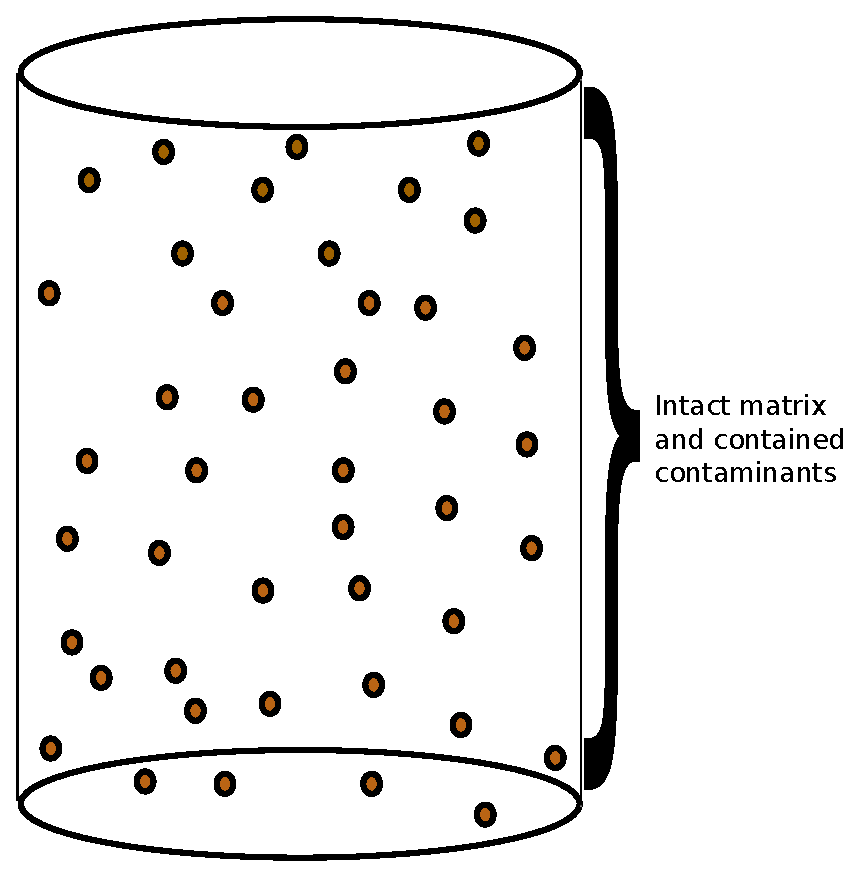
\includegraphics[width=0.9\linewidth]{mixed_cell/mixed_cell_whole.eps}
  \end{center}
  \caption[Intact Mixed Cell Control Volume]{The control volume contains an 
  intact material matrix. Contaminants are unavailable to neighboring 
  subcomponents until dissolution has begun.}
  \label{fig:intact}
\end{minipage}
\hspace{0.5cm}
\begin{minipage}[b]{0.5\linewidth}
  \begin{center}
    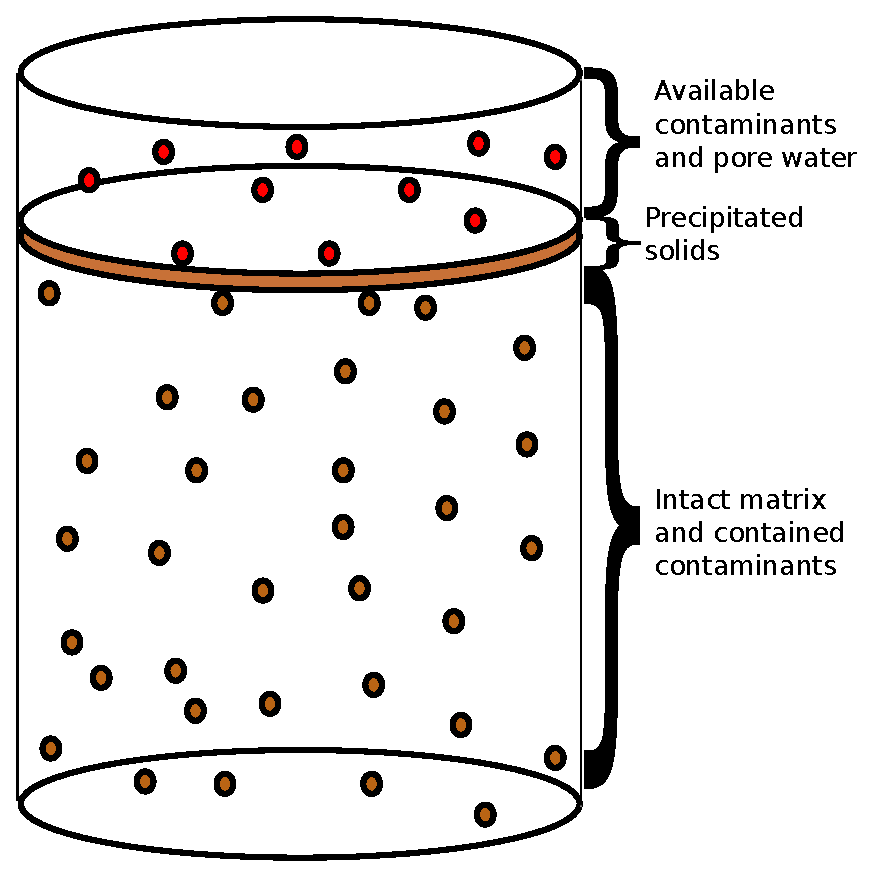
\includegraphics[width=0.9\linewidth]{mixed_cell/mixed_cell_degraded.eps}
  \end{center}
  \caption[Degrading Mixed Cell Control Volume]{Once dissolution begins, the 
  control volume contains a partially dissolved material matrix, contaminated 
  pore water, and precipitated solids.}
  \label{fig:dissolved}
\end{minipage}
\end{figure}


After some time degrading, the volume of free fluid can be expressed as
\begin{align}
V_{ff}(t_n) &= \theta V_T \int_{t_0}^{t_n} f(\cdots) dt.
\label{vff}
\end{align}

The volume of the intact matrix can be expressed as
\begin{align}
V_{im}(t_n) &= V_T - V_T\int_{t_0}^{t_n} f(\cdots) dt.
\label{vim}
\end{align}

Finally, the volume of the precipitated solids can be expressed as
\begin{align}
V_{ps}(t_n) &= (1 - \theta)V_T\int_{t_0}^{t_n} f(\cdots) dt.
\label{vps}
\end{align}

This model assumes that all net influx to the cell enters the free fluid rather 
than the intact matrix. The total volumetric contaminant concentration in the intact matrix, 
can be expressed as

\begin{align}
C_{im}(t_n) &= C_0\\
            &= \frac{m_0}{V_{im}(t_0)}
\intertext{where}
%here we assume nothing escapes an intact matrix
m_0 &= \mbox{ total initial mass. } \nonumber
\end{align}

The resulting contaminant mass in the intact matrix at time $t_n$ is 

\begin{align}
m_{im}(t_n) &= C_0 V_{im}(t_n)\nonumber\\
            &= C_0V_T\left(1-\int_{t_0}^{t_n}f(\cdots)dt\right). 
\label{mim}
\end{align}

The contaminant mass in the free fluid is just the initial pore water concentration 
times the free fluid volume plus the time integral of net influx to the cell
such that

\begin{align}
C_{ffT}(t_n) &= \left[C_0 + \frac{\int_{t_0}^{t_n} \dot{m}_{i}(t') dt'}{V_{ff}(t_n)}\right] 
\intertext{and}
m_{ffT}(t_n) &= C_{ff}(t_n) V_{ff}(t_n)\nonumber\\
       &= \left[C_0 + \frac{\int_{t_0}^{t_n} \dot{m}_{i}(t') dt'}{V_{ff}(t_n)}\right] V_{ff}(t_n) \nonumber\\
       &= C_0V_{ff}(t_n) + \int_{t_0}^{t_n} \dot{m}_{i} dt'.
\end{align}

It is limited, however, by both solubility limitation and sorption. 

\subsubsection*{Sorption}

The mass in both the free fluid and in the intact matrix exists in both 
sorbed and non-sorbed phases. The relationship between the sorbed mass 
concentration in the solid phase (e.g. the pore walls),

\begin{align}
s &=\frac{\mbox{ mass of sorbed contaminant} }{ \mbox{mass of total solid phase }}
\label{solid_conc}
\end{align}
and the dissolved liquid concentration, 
\begin{align}
c &=\frac{\mbox{ mass of dissolved contaminant} }{ \mbox{volume of total liquid phase }}
\label{liquid_conc}
\end{align}
can be expressed by a number of isotherm models.

In this model, sorption is taken into account throughout the volume. In the 
intact matrix, the contaminant mass is distributed between the pore walls and 
the pore fluid by sorption.  So too, contaminant mass released from the intact 
matrix by degradation is distributed between dissolved mass in the free fluid 
and sorbed mass in the precipitated solids.

To solve for the boundary condiitons in this model, the amount of non-sorbed 
contaminant mass in the free fluid must be found. This value, $m_{ffl}$, can be 
expressed in terms of the total degraded contaminant mass and the contaminant 
mass in the precipitated solid,

\begin{align}
m_{ffl} &= m_{ffT} - m_{psc}.
\label{m_ffl}
\end{align}

The mass of contaminant sorbed into the precipitated solids can be found using a 
linear isotherm model \cite{schwartz_fundamentals_2003}, characterized by the relationship 
\begin{align}
s_{i} &= K_{di} c_{i}
\label{linear_iso}
\intertext{where}
s_i &= \mbox{ the solid concentration of isotope i }[kg/kg]\nonumber\\
K_{di} &= \mbox{ the distribution coefficient of isotope i}[m^3/kg]\nonumber\\
c_i &= \mbox{ the liquid concentration of isotope i }[kg/m^3].\nonumber
\end{align}

Thus, from \eqref{solid_conc},

\begin{align}
s_{i,ps} &= \frac{\mbox{contaminant mass in precipitated solids} }{ \mbox{total mass of precipitated solids}}\nonumber\\
         &= \frac{m_{psc}}{m_{psT}}\nonumber\\
         &= \frac{m_{psc}}{m_{psm} + m_{psc}}\nonumber
\intertext{where}
m_{psm}  &= \mbox{ noncontaminant mass in precipitated solids }[kg]\nonumber\\
         &= \rho_bV_{ps}\nonumber\\
m_{psc}  &= \mbox{ contaminant mass in precipitated solids }[kg]\nonumber\\
\rho_b   &= \mbox{ bulk (dry) density of the medium }[kg/m^3].\nonumber\\
\end{align}

The following expression results, giving contaminant mass in the precipitated 
solids in terms of the sorption coefficient,
\begin{align}
m_{psc} &= s_{ps}m_{psT}\nonumber\\
          &= K_dC_{ffl}m_{psT}\nonumber\\
          &= \frac{K_dm_{ffl}m_{psT}}{V_{ff}}\nonumber\\
          &= \frac{K_d}{V_{ff}}(m_{ffT}-m_{psc})m_{psT}\nonumber\\
          &= \frac{K_d}{V_{ff}}(m_{ffT}-m_{psc})(m_{psm}+m_{psc})\nonumber\\
          &= \frac{K_d}{V_{ff}}(m_{ffT}m_{psm}-m_{psc}m_{psm} + m_{ff}m_{psc} -m_{psc}^2)\nonumber\\
          &= \frac{K_d}{V_{ff}} (m_{ffT}m_{psm} + (m_{ffT} - m_{psm})m_{psc} - m_{psc}^2)\nonumber
\intertext{which, rearranged, becomes }
0         &= m_{psc}^2 + \left( -m_{ffT} + m_{psm} + \frac{V_{ff}}{K_d} \right)m_{psc} - m_{ffT}m_{psm}\nonumber
\intertext{and is solved using the quadratic formula, such that}
m_{psc}   &= \frac{m_{ffT} - m_{psm} - \frac{V_{ff}}{K_d}}{2}
             \pm\frac{\sqrt{\left(-m_{ffT} + m_{psm} + \frac{V_{ff}}{K_d}\right)^2 -4m_{ffT}m_{psm}}}{2}\nonumber\\  
          %&= \frac{m_{ffT} - m_{psm} - \frac{V_{ff}}{K_d}}{2} \nonumber\\
          %& \pm\frac{\sqrt{m_{ffT}^2 + m_{psm}^2 + \frac{V_{ff}^2}{K_d^2} + 2m_{ffT}m_{psm} - 
          %   \frac{2V_{ff}m_{ffT}}{K_d} + \frac{2V_{ff}m_{psm}}{K_d} } }{2} \nonumber
\intertext{which, again rearranged, becomes}
          &= \frac{1}{2} \left(m_{ffT} - m_{psm} - \frac{V_{ff}}{K_d}\right) \nonumber\\
          & \pm \frac{1}{2} \sqrt{m_{ffT}^2 + 2m_{ffT}\left(m_{psm} - 
          \frac{V_{ff}}{K_d}\right) + \left(m_{psm} + 
          \frac{V_{ff}}{K_d}\right)^2}.
\label{m_psc}
\end{align}

Plugging \eqref{m_psc} into \eqref{m_ffl} results in the 
following expression for $m_{ffl}$ in terms of known quantities

\begin{align}
m_{ffl}   &= m_{ffT} - \frac{1}{2} \left(m_{ffT} - m_{psm} - \frac{V_{ff}}{K_d}\right) \nonumber\\
          & \mp \frac{1}{2} \sqrt{m_{ffT}^2 + 2m_{ffT}\left(m_{psm} - 
          \frac{V_{ff}}{K_d}\right) + \left(m_{psm} + 
          \frac{V_{ff}}{K_d}\right)^2}.
\label{m_ffl_full}
\end{align}


\subsubsection*{Solubility}
  In addition to engineered barriers, contaminant movement is constrained by 
  the solubility limit \cite{hedin_integrated_2002}, 
    \begin{align}
      m_{s,i} &\leq V_w C_{sol,i},
    \intertext{where}
      m_{s,i} &= \mbox{ solubility limited mass of isotope i in volume }V_w [kg]\nonumber\\ 
      V_w &= \mbox{ volume of the solution }[m^3]\nonumber\\
      C_{sol,i} &= \mbox{ solubility limit, the maximum concentration of i }[kg/m^3].\nonumber
    \end{align}


The desired boundary conditions can be expressed in terms of $m_{ffl}$. First, the 
Dirichlet boundary condition is 
\begin{align}
C(x,y,z,t) = \frac{m_{ffl}(t)}{V_{ff}(t)}\forall (x,y,x) \in \Gamma.
\label{dirichlet_mixed}
\end{align}

From this boundary condition in combination with global advective velocity 
data, all other boundary conditions can be found. 


\subsection*{Lumped Parameter Radionuclide Model}\label{sec:lumped}

The response function model implemented interchangeable piston flow, 
exponential, and dispersion response functions and was developed by direct 
calibration against the results of the abstraction effort.  


\subsubsection*{One Dimensional Permeable Porous Medium Radionuclide Transport 
Model}\label{sec:one_dim_ppm}
Finally, abstraction results informed modifications to the implementation of an 
analytic solution to the one dimensional advection-dispersion equation with 
finite domain and Cauchy and Neumann boundary conditions at the inner and outer 
boundaries, respectively. 

Various solutions to the advection dispersion equation  
\eqref{unidirflow} have been published for both the first and third types of 
boundary conditions. The third, Cauchy type, is mass conservative, and will be 
the primary kind of boundary condition used at the source for this model.

The conceptual model in Figure \ref{fig:1dinf} represents solute transport
in one dimension with unidirectional flow and a semi-infinite boundary condition 
in the positive flow direction. 

The solution is given (Leij and van Genuchten, \cite{leij_analytical_1991})  as :
\begin{align}
  \end{align}

\vspace{1cm}
\begin{figure}[htbp!]
  \begin{center}
    \def\svgwidth{.5\textwidth}
    \input{one_dim_ppm/1dinf.eps_tex}
  \end{center}
  \caption{A one dimensional, semi-infinite model, unidirectional flow,
  solution with Cauchy and Neumann B.C.s}
  \label{fig:1dinf}
\end{figure}

With the boundary conditions
\begin{align}
  -D \frac{\partial C}{\partial x}\big|_{x=0} + v_xc &= \begin{cases}
    vC_0  &  \left( 0<t<t_0 \right)\\
    0  &  \left( t>t_0 \right)\\
  \end{cases}\\
  \frac{\partial C}{\partial x}\big|_{x=\infty} &= 0
  \intertext{and the initial condition}
  C(x,0) &= C_i,
  \label{1dinfBC}
  \intertext{the solution is given as }
  C(x,t) = \frac{C_0}{2}\Bigg[&\erfc{\frac{L-v_xt}{2\sqrt{D_Lt}}} 
  + \frac{1}{2} \left(\frac{v_x^2t}{\pi D_L}\right)^{1/2}e^{\frac{-( L - 
  v_xt)^2}{4D_Lt}}\nonumber\\
  &- \frac{1}{2}\left( 
  1+\frac{v_xL}{D_L}+\frac{v_x^2t}{D_L}\right)e^\frac{v_xL}{D_L}\erfc{\left[\frac{L-V_xt}{2\sqrt{D_Lt}}\right]} 
  \Bigg]
\end{align}





\section*{DISCUSSION OF THE BASE CASE DEMONSTRATION}

A base case simulation was conducted as a proof of principle demonstration of 
the modularity and interchangeability of these models. The simplest of the 
contaminant transport models was used to represent the natural and engineered 
barrier components of a repository concept. This concept consisted of a  
saturated clay environment.  In this demonstration, the \Cyder open source 
library integrates with the Cyclus computational fuel cycle systems analysis 
platform in order to calculate repository performance metrics with respect to 
candidate fuel cycle options.  Thus, the demonstration illuminates the 
suitability of \Cyder's interface for linking to other tools as well as for use 
as a stand-alone radionuclide transport calculation engine.

The demonstration case is an empty software architecture in which to implement 
the physical models. This demonstration has built and tested component module 
loading of models and data, information passing between components represented by 
degradation rate nuclide transport models, and database writing.

Results of unit tests and benchmarking efforts were positive as was a proof of 
principle base case demonstration of the interface between these models. The 
base case demonstration has used the degradation rate to represent nuclide 
transport through waste form, waste package, and buffer components in a generic, 
isotropic, permeable porous geological medium with reducing geochemistry as well 
as the near field. Expected degradation behavior and congruent release was 
observed in unit testing.  

  \begin{figure}[htbp!]
    \begin{center}
      \includegraphics[width=.5\textwidth]{base_case/componentLoading.eps}
      \caption{Waste form, waste package, buffer, and far field components 
        posess transport behavior selected from available transport 
        models, are parameterized by user data, and are loaded modularly 
      into a cohesive framework.}
    \end{center}
  \end{figure}

  \input{base_case/base_case_table}


\section*{CONCLUDING REMARKS}
The Cyder source code in which these models are implemented as well as 
associated documentation are freely available to interested researchers and 
potential model developers. The application programming interface to this 
software library is intentionally general, facilitating the incorporation of the 
models presented here within external software tools in need of a multicomponent 
repository model.

Furthermore, this work contributes to an expanding ecosystem of computational 
models available for use with the Cyclus fuel cycle simulator. This hydrologic 
nuclide transport library, by virtue of its capability to modularly integrate 
with the Cyclus fuel cycle simulator has laid the foundation for integrated 
disposal option analysis in the context of fuel cycle options. 


\bibliographystyle{plain}
\bibliography{paper}
\end{document}


